% !TeX TXS-program:compile = txs:///pdflatex/[--shell-escape]
\documentclass[11pt,a4paper]{exam}
\printanswers % pour imprimer les réponses (corrigé)
%\noprintanswers % Pour ne pas imprimer les réponses (énoncé)
\addpoints % Pour compter les points
\usepackage[utf8]{inputenc}
\usepackage{minted}

%\usepackage[margin=1 in]{geometry}
\usepackage[a4paper,top=2.5cm,bottom=2.5cm,left=1.5cm,right=1.5 cm,marginparwidth=1.75cm]{geometry}
\usepackage{amsmath,amssymb}
\usepackage{multicol}
\usepackage{graphicx}
\usepackage{setspace}
\usepackage{dashundergaps}

% Pour afficher des numéros de ligne dans verbatim
\usepackage{listings}
\lstset{
	basicstyle=\ttfamily, % Set the basic style to typewriter font
	numbers=left,         % Position line numbers on the left
	numberstyle=\tiny,    % Set the style of the line numbers
	stepnumber=1,         % Line number increment
	numbersep=5pt,        % How far the line numbers are from the code
	%frame=single,         % Adds a frame around the code
	tabsize=2,            % Sets default tabsize to 2 spaces
	breaklines=true,      % Enables line breaking
	breakatwhitespace=false, % Break lines not only at whitespaces
}


\newcommand{\examnum}{Contrôle majeur \#2}
\newcommand{\class}{SNT 2\textsuperscript{nde}}
\newcommand{\examdate}{15/01/2024}
\newcommand{\timelimit}{45 Minutes}
\newcommand{\lycee}{Lycée Fustel de Coulanges}

\pagestyle{head}
\firstpageheader{}{}{}
\runningheader{\class}{\examnum\ - Page \thepage\ / \numpages}{\examdate}
\runningheadrule


\begin{document}
% Espace d'en-tête
\noindent
\begin{spacing}{1}
	\noindent
	\begin{tabular*}{\textwidth}{l @{\extracolsep{\fill}} l @{\extracolsep{6pt}} l}
		\textbf{\class} & \textbf{\examnum, \examdate}&\\
		\textbf{\lycee} &\textbf{Durée: \timelimit} &\\
	\end{tabular*}\\
\end{spacing}

\noindent
\vspace{10pt}
\hrule
\vspace{5pt} 
\noindent
\\
Ce contrôle comporte \numquestions\ questions; le maximum possible de points est de \numpoints\ points.\\ 
Les réponses sont à porter sur une \uline{\textbf{copie}} (\textbf{PAS} un morceau de papier arraché d'un cahier ou une copie déchirée) \uline{comportant votre nom}.\\
Il n'est pas nécessaire de répondre aux questions dans l'ordre \textemdash\ commencez par celles où vous vous sentez le plus à l'aise (mais numérotez bien les questions sur votre copie).\\
Les calculatrices ne sont \uline{pas} autorisées.\\
\noindent
\hrule
\vspace{15pt} 

    \begin{spacing}{1,1}
        \begin{questions} % DEBUT DE L'EXAMEN
        	
        	\question QCM -- reportez sur votre copie la ou les réponses correctes \textit{en mentionnant bien la lettre de la question à chaque fois}.
			\begin{parts}
				\part[1]Le code RVB 0-255-0 correspond à la couleur:
        			\begin{choices}
		        			\choice Jaune.
		        			\choice Rouge.
		        			\correctchoice Verte.
		        			\choice Noire.
        			\end{choices}
        		\part[1]Coder une couleur sur 4 bits permet de différencier:
	        		\begin{choices}
	        			\choice 2 couleurs.
	        			\choice 4 couleurs.
	        			\choice 8 couleurs.
	        			\correctchoice 16 couleurs.
	        			\choice 32 couleurs.
	        		\end{choices}
        		\part[1]Le langage HTML sert à:
	        		\begin{choices}
	        			\correctchoice Structurer et présenter le contenu sur les pages Web.
	        			\choice Protéger les sites web contre les hackers.
	        			\correctchoice Décrire la structure de base d'un document sur Internet
	        			\choice Créer et gérer des bases de données.
	        			\choice Toutes les réponses ci-dessus sont vraies.
	        		\end{choices}
			\end{parts}
			        	
        	\question[2] Si vous désactivez les cookies dans votre navigateur, quel impact cela pourrait-il avoir sur votre navigation sur Internet ? Donnez un exemple concret (en citant un site web spécifique et au moins deux conséquences précises).
			\begin{solution}
        		Tout ou partie des éléments de réponse suivants étaient attendus:
        		\begin{itemize}
        			\item Fonctionnalités limitées sur le site web:
        			\begin{itemize}
        				\item Perte des éléments de préférences -- la langue par défaut sera affichée (si une autre avait été choisie elle n'aura pas été enregistrée); sur un site d'informations par exemple les catégories préférées ne seront pas affichées; etc...
        				\item Perte d'historique: par exemple, si un panier d'achats avait été constitué lors d'une visite précédente il aura été perdu.
        			\end{itemize}
        			\item Amélioration de la confidentialité: le suivi de votre comportement en ligne sera beaucoup plus difficile pour les annonceurs partenaires du site web visité. 
        			\item Parfois, impact sur les performances du site web -- le site visité ne peut pas optimiser votre visite en fonction de vos visites précédentes et des informations que vous aviez fournies.
        			\item Dans certains cas, impossibilité complète de visiter un site web -- certains sites imposent l'utilisation de cookies et donc vous refusent l'accès si vous les désactivez.
        		\end{itemize}
        	\end{solution}
        	
        	\question[2] Un ami vous appelle en panique car il pense que son ordinateur a été infecté par un logiciel malveillant. Quels trois conseils pratiques lui donneriez-vous pour gérer la situation et protéger ses données?
        	\begin{solution}
        		Tout ou partie des éléments de réponse suivants étaient attendus:
        		\begin{itemize}
        			\item Se déconnecter d'internet;
        			\item Exécuter un diagnostic et si possible un nettoyage au moyen d'un logiciel anti-virus;
        			\item Eventuellement redémarrer votre système d'exploitation (Windows, Linux, MacOS...) en mode "sans échec";
        			\item S'il s'agit d'un ransomware (donc avec une demande de somme d'argent associée pour récupérer ses données), surtout ne pas payer;
        			\item Si vraiment la situation semble désespérée, faire appel à un professionnel -- sachant que a) il n'est pas certain qu'il ou elle puisse résoudre le problème, et b) la prestation sera payante;
        			\item Une fois la situation résolue, changer ses mots de passe sur tous les sites web; mettre à jour le logiciel antivirus, le système d'exploitation; bien vérifier que toutes ses données sont sauvegardées; etc...
        		\end{itemize}
        	\end{solution}
        		
        	
        	\question[2] Imaginons que la neutralité du net a été abolie: expliquez (en donnant trois exemples concrets en tout) les conséquences possibles d'une telle mesure -- pour vous, en tant qu'utilisateur d'internet, et pour une petite entreprise / startup de vente en ligne.
			\begin{solution}
				Tout ou partie des éléments de réponse suivants étaient attendus:
				\begin{itemize}
					\item Pour vous, en tant qu'utilisateur internet:
					\begin{itemize}
						\item Si par exemple vous vous aimez regarder des vidéos en streaming, ces services pourraient devenir plus lents (et donc saccadés ou de basse qualité) à moins de payer un supplément à votre FAI.
						\item Une version différente de la conséquence précédente pourrait être que votre FAI, sans vous proposer de payer de supplément, dégrade l'accès (voire le bloque complètement) à certains sites avec lesquels il n'est pas partenaire, vous obligeant à en utiliser d'autres.
						\item Plus généralement le coût d'accès au contenu internet augmentera puisque le coût qu'imposeront les FAI sur les fournisseurs de contenu sera en toute logique répercuté sur l'utilisateur final.
					\end{itemize}
					\item Pour une petite entreprise de vente en ligne - et ces points sont les pendants de ceux pour les utilisateurs:
					\begin{itemize}
						\item Une startup pourrait se voir contrainte de payer des frais au FAI pour que  ses services soient chargés rapidement;
						\item Si le produit que propose la startup est en concurrence avec un du FAI lui-même ou d'un de ses partenaires, le FAI pourrait refuser de donner accès au service de la startup ou en tous cas de le limiter beaucoup;
						\item Au bilan une startup aurait vraisemblablement beaucoup de frais en plus qu'actuellement qu'elle devrait soit absorber soit répercuter sur ses clients -- rendant ainsi ses produits ou services plus chers et donc moins attractifs.
					\end{itemize}
				\end{itemize}
			\end{solution}
        	
        	\question[2] "\textit{Les moteurs de recherche coome Google, ça fonctionne parfaitement: on pose une question, ça nous donne la meilleure réponse possible, et c'est absolument tout.}" Donnez deux arguments qui pourraient aller à l'encontre d'une telle affirmation.
        	\begin{solution}
        		Tout ou partie des éléments de réponse suivants étaient attendus:
        		\begin{itemize}
        			\item "Bulles de filtres": les moteurs de recherche personnalisent souvent les résultats de recherche en fonction de l'historique de navigation, de la localisation, et d'autres données personnelles de l'utilisateur - la réponse que fournit un moteur de recherche n'est donc généralement pas "la" bonne réponse mais une dont l'algorithme a déterminé qu'elle plairait à l'utilisateur, renforçant ainsi potentiellement ses biais.
        			\item Fonctionnement du référencement: par les techniques de SEO (Search Engine Optimization) les sites ont la capacité de mettre en avant leurs contenus dans les moteurs de recherche -- or ce SEO est une technique commerciale, absolument pas un garant de qualité de contenu;
        			\item Contenu sponsorisé: souvent, les moteurs de recherche mettent en tête de la liste des réponses qu'ils proposent du contenu de sites qui les rémunèrent -- là encore c'est le résultat d'une démarche commerciale, pas d'un filtrage de qualité de contenu.
        			\item Plus généralement les moteurs de recherche savent évaluer des éléments mesurables (nombre de visites d'un site par exemple, ou mots clés fournis par les sites), mais n'ont pas la capacité de déterminer la fiabilité ou la véracité d'un contenu -- pour faire simple, un résultat d'une recherche peut tout à fait être factuellement faux.
        		\end{itemize}
        	\end{solution}
        	
        	\question[2] Une de vos amies, résidant en France, a trouvé lors d'une recherche Google de vieux articles négatifs la concernant publiés sur un site américain. Ces articles décrivaient des faits qui étaient vrais il y a longtemps mais qui ne le sont plus actuellement. Elle craint que cette cela nuise à sa recherche d'emploi et souhaite qu'ils soient supprimés. Elle vous demande votre avis: que lui conseillez-vous? Quels sont ses droits en termes de suppression de ces informations selon la législation, notamment le RGPD?
        	\begin{solution}
        		Tout ou partie des éléments de réponse suivants étaient attendus:
        		\begin{itemize}
        			\item Le premier conseil est de voir si une solution peut être trouvée sans passer par des voies légales -- si l'amie contacte le site web et leur demande poliment de retirer le contenu, il se peut tout à fait qu'ils acceptent!
        			\item Elle peut cependant aussi s'appuyer sur le droit à l'oubli inscrit dans le RGPD -- ça ne pourra pas s'appliquer au site web dans ce cas (puisqu'il est américain et que le RGPD est un règlement de l'Union Européenne) mais cela pourra tout au moins s'imposer aux moteurs de recherche qui devront (si la décision de justice est conforme aux espoirs de votre amie évidemment) désindexer le contenu pour les recherches effectuées dans l'UE, le rendant ainsi moins accessible.
        		\end{itemize}
        	\end{solution}
        	
        	\question Considérez le code HTML suivant:
        	\begin{lstlisting} % Verbatim numéroté au moyen du package listings

<!DOCTYPE html>
<html lang="fr">
    <head>
        <title>Ma page HTML
    </head>
    <body>
        <h1>Mes gouts</h1>
        <h2>La lecture</h2>
        <img src="livre.jpg">
        <br /> <br /> <br />
        Ce que j'aime lire:
        <ul>
            <li>Des livres</a></li>
            <li><a www.lemonde.fr>Le journal</a></li>
        <FinDeListe>
        <h2>Le sport</h2>
    </body>
</html>
        	\end{lstlisting}
        	
        	\begin{parts}
        		\part[2] Ce code contient plusieurs erreurs: identifiez-en au moins deux et expliquez comment il faut les corriger.
        		\begin{solution}
        			Plusieur erreurs ici:
        			\begin{itemize}
        				\item Ligne 4: la balise \texttt{<title>} n'est pas fermée (il manque \texttt{</title>});
        				\item Ligne 13: une balse \texttt{a} est fermée (\texttt{</a>}) alors qu'elle n'a jamais été ouverte;
        				\item Ligne 14: la balise de lien \texttt{a} est mal formée -- il manque le nom de l'attribut "lien" qui est \texttt{href}. La syntaxe correcte serait:
        				\texttt{<a href="http://www.lemonde.fr">Le journal</a>}
        				\item Ligne 15: la balise \texttt{<FinDeListe>} n'existe pas en HTML;
        				\item Ligne 15: la balise de liste \texttt{ul} n'a pas été fermée -- il manque ici \texttt{</ul>}.
        			\end{itemize}
        			Ce code corrigé ressemblerait alors à:
        			\begin{lstlisting}
<!DOCTYPE html>
<html lang="fr">
    <head>
        <title>Ma page HTML</title>
    </head>
    <body>
        <h1>Mes gouts</h1>
        <h2>La lecture</h2>
        <img src="livre.jpg">
        <br><br><br>
        Ce que j'aime lire :
        <ul>
            <li>Des livres</li>
            <li><a href="http://www.lemonde.fr">Le journal</a></li>
        </ul>
        <h2>Le sport</h2>
    </body>
</html>
				\end{lstlisting}

        		\end{solution}
        		\part[1] En supposant que le code a été corrigé, dessinez sur votre copie le rendu qu'aurait cette page dans un navigateur web comme Firefox par exemple.
        		\begin{solution}
        			En supposant bien sûr qu'une image "livre.jpg" existe bien, l'aspect de cette page serait:
        			
        			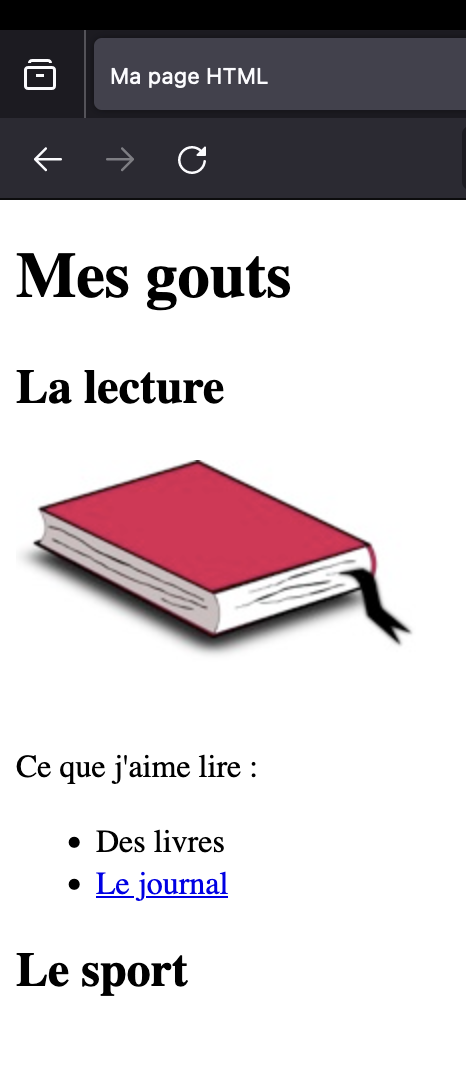
\includegraphics[scale=0.5]{PageHTML.png}
        		\end{solution}
        		\part[1] En supposant toujours que le code a été corrigé, où s'afficherait le texte "Ma page HTML"?
        		\begin{solution}
        			Comme on peut le voir dans la représentation ci-dessus, "Ma Page HTML" est le titre de cette page et s'affiche donc dans l'onglet du navigateur, au-dessus de la page elle-même.
        		\end{solution}
        	\end{parts}
        		
			\question[2 \half] Considérez le texte suivant:
			
			\textit{Dans un appareil photo numérique, la lumière passe à travers \uline{\ \ \ \ }\textbf{(A)}\uline{\ \ \ \ } et frappe le \uline{\ \ \ \ }\textbf{(B)}\uline{\ \ \ \ }, qui est composé de millions de \uline{\ \ \ \ }\textbf{(C)}\uline{\ \ \ \ } sensibles à la lumière; chacun de ces \uline{\ \ \ \ }\textbf{(C)}\uline{\ \ \ \ } convertit la lumière en un signal analogique, puis un signal numérique dans lequel l'image est découpée en \uline{\ \ \ \ }\textbf{(D)}\uline{\ \ \ \ }, avant d'être stockée dans la \uline{\ \ \ \ }\textbf{(E)}\uline{\ \ \ \ } de l'appareil pour une visualisation ultérieure.}
			
			Donnez les mots manquants dans ce texte -- de \textbf{(A)} à \textbf{(E)}.
			
			\begin{solution}
				Les mots manquants étaient:
				\begin{itemize}
					\item[ A: ] l'objectif
					\item[ B: ] capteur
					\item[ C: ] photosites \textit{(qui apparaissait donc deux fois dans le texte)}
					\item[ D: ] pixels
					\item[ E: ] mémoire
				\end{itemize}
			\end{solution}
			
			\question On considère une image numérique de forme carrée de 1000 pixels de côté, que l'on imprime sur une feuille 10 pouces (environ 25 cm) de côté.
			
			\begin{parts}
				\part[1] Quelle est la définition de cette image?
				\begin{solution}
					La définition d'une image est le nombre de pixels dont elle est constituée -- dans ce cas on a un carré de 1000 pixels de côtés, donc $1000 \times 1000 = 1000000$ de pixels, autrement dit "1 mégapixel".
				\end{solution}
				\part[1] Sa résolution?
				\begin{solution}
					La résolution d'une image (imprimée ou affichée sur un écran) s'exprime en pixels par pouce ("ppp") et est calculée selon la formule:
					
					$ \text{résolution} = \frac{\text{nombre de pixels}}{\text{taille de l'impression en pouces}} $
					
					Dans notre cas on aura donc:
					
					$ \text{résolution} = \frac{1000}{10} = 100 \text{ ppp}$
				\end{solution}
				\part[\half] Combien devrait mesurer le côté de la feuille pour atteindre une résolution de 400 ppp?	
				\begin{solution}
					Partant d'une résolution de 100 ppp on veut en atteindre une de 400, en modifiant la taille de l'impression (le nombre de pixels, soit la définition, ne peut jamais être augmenté -- il est fixé au moment de la prise de vue). Pour quadrupler une valeur en modifiant le dénominateur d'une fraction il faut bien sûr diviser ce dénominateur par quatre. Le côté de la feuille devrait donc mesurer $10 / 4 = 2,5$ pouces (soit un peu plus de 6 centimètres).
				\end{solution}			
			\end{parts}
  
        \end{questions}
    \end{spacing}
\end{document}